%%%%%%%%%%%%%%%%%%%%%%%%%%%%%%%%%%%%%%%%%
% University/School Laboratory Report
% LaTeX Template
% Version 3.1 (25/3/14)
%
% This template has been downloaded from:
% http://www.LaTeXTemplates.com
%
% Original author:
% Linux and Unix Users Group at Virginia Tech Wiki 
% (https://vtluug.org/wiki/Example_LaTeX_chem_lab_report)
%
% Modified by:
% Riccardo Prinzivalle
%
% License:
% CC BY-NC-SA 3.0 (http://creativecommons.org/licenses/by-nc-sa/3.0/)
%
%%%%%%%%%%%%%%%%%%%%%%%%%%%%%%%%%%%%%%%%%

%----------------------------------------------------------------------------------------
%	PACKAGES AND DOCUMENT CONFIGURATIONS
%----------------------------------------------------------------------------------------

\documentclass{article}

\usepackage{graphicx} % Required for the inclusion of images
\usepackage[square,numbers]{natbib} % Required to change bibliography style to APA
\usepackage{amsmath} % Required for some math elements 
\usepackage[hyphens]{url} % required for url in bibliography
\usepackage{hyperref} % required for hyperlink in url
\usepackage{float} % required for positioning of table
\usepackage{pdflscape} % required for table rotation
\usepackage{array, makecell} % for multiline cells of table
%\usepackage{tabularx}
%\newcolumntype{L}{>{\raggedright\arraybackslash}X}

\setlength\parindent{0pt} % Removes all indentation from paragraphs

%\usepackage{times} % Uncomment to use the Times New Roman font

%----------------------------------------------------------------------------------------
%	DOCUMENT INFORMATION
%----------------------------------------------------------------------------------------

\title{Implementation of SED with Depthwise Separable and Dilated Convolutions \\[0.2em]\small{}Neural Networks Sapienza 2020} % Title

\author{Riccardo \textsc{Prinzivalle}} % Author name

\date{March 2021} % Date for the report

\begin{document}

\maketitle % Insert the title, author and date

%\begin{abstract}
%Some abstract text for presentation
%\end{abstract}

%----------------------------------------------------------------------------------------
%	SECTION 1
%----------------------------------------------------------------------------------------

\section{Introduction}
\label{sec:intro}

This project is a study and implementation of a polyphonic sound event detection extracted from \cite{drossos2020sound}. It is also based on the baseline reference of \cite{drossos2020sound}, which is \cite{Cakir_2017}. These two works represent the main source of this project. Here there will be presented both a replication of the paper approach together with a monophonic sound event detection, since to obtain the original dataset took some time, the author thought to start working with another dataset and then move the work to the original dataset when it would have been available. Section \ref{sec:mono} and \ref{sec:poly} are organized as follows: first an analysis of the dataset is performed to better understand it, then it is explained how the feature have been extracted and finally it is proposed a model to solve the problem. Section \ref{sec:results} regroups the results for both datasets, then it is explained a brief digression on how to train a neural network model on an AMD GPU on section \ref{sec:AMD} since the author's setup has only an AMD GPU. The work is ended by conclusions of section \ref{sec:end}.
 
%----------------------------------------------------------------------------------------
%	SECTION 2
%----------------------------------------------------------------------------------------

\section{Monophonic SED}
\label{sec:mono}

Monophonic Sound Event Detection consist of predicting a single label for an audio recording: the record will likely contain some noise but it generally contains a single and remarkable sound to be identified. In this case, it is used the \textit{UrbanSound8K} dataset \cite{Salamon:UrbanSound:ACMMM:14}.

\subsection{Data analysis}
\label{subsec:mono_analysis}

The dataset is composed by 8732 labelled small sound recordings (less than 4 seconds) from 10 classes: \textit{air\_conditioner}, \textit{car\_horn}, \textit{children\_playing}, \textit{dog\_bark}, \textit{drilling}, \textit{engine\_idling}, \textit{gun\_shot}, \textit{jackhammer}, \textit{siren}, and \textit{street\_music}. The classes are balanced except for some, it can be seen in table \ref{tab:mono_distribution}. Only 3 out of 10 classes have less than 1000 elements, so there can be some problems predicting these classes.

\begin{table}[H]
	\begin{center}
		\begin{tabular}{ |c | c | }
			\hline
			Label & number of elements \\ 
			\hline
			air\_conditioner & 1000 \\
			\hline
			car\_horn & 429 \\
			\hline
			children\_playing & 1000 \\
			\hline
			dog\_bark & 1000 \\
			\hline
			drilling & 1000 \\
			\hline
			engine\_idling & 1000 \\
			\hline
			gun\_shot & 374 \\
			\hline
			jackhammer & 1000 \\
			\hline
			siren & 929 \\
			\hline
			street\_music & 1000 \\
			\hline
		\end{tabular}
		\caption{Monophonic dataset label distribution}
		\label{tab:mono_distribution}
	\end{center}
\end{table}

Moreover, the recordings have different properties since the come from \href{www.freesound.org}{} and are taken as they are. The first difference is in the audio lengths visible in figure \ref{fig:mono_duration}: the majority of audio have a duration of about 3.5/4 seconds, but there exists also smaller recordings which are in a tiny number.

\begin{figure}[H]
	\centering
	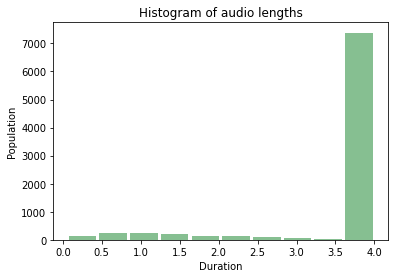
\includegraphics[width=0.8\textwidth]{./images/mono/duration.png}	
	\caption{Audio duration distribution}
	\label{fig:mono_duration}
\end{figure}

The main differences are in bit depth, from 4 to 32 bit, the majority with 16 bit; and in the sample rate, from 8 KHz to 192 KHz, with the majority with 44.1 KHz. This may be a concern since some audio have a poor quality which can translate in poorer feature w.r.t. the other tracks. All these differences will be equalized during the feature extraction phase.

\subsection{Feature Extraction}
\label{subsec:mono_feature}

This phase adopts librosa \cite{mcfee2015librosa}, which is a sound processing library for python. Its use helps to deal with different audio characteristics since by default librosa converts audio to 22 KHz sampling rate and 16 bit depth. Since the majority of audio recordings are at 44.1 KHz, it may seem that down sampling may reduce audio quality, but if we visualize the sound with a spectrogram, it will be clear that most of frequency content is distributed well below the 11 KHz (which is the maximum frequency a 22 KHz sampling rate can process), so in this case it reduces the dimension of the data without losing much information. For what concerns the bit depth, the majority of recordings are already at 16 bit, so it does not change much the data. Audio file are loaded and transformed into array series by \textit{load} function, which is also responsible of audio conversion and standardization.\newline
The reference paper \cite{drossos2020sound} uses Mel Frequency Cepstral Coefficients (MFCC) to extract features from the array sound data. MFCCs are a way of measuring the rate of information change in spectral bands and storing it in coefficients; moreover, the rate of change is modeled in a non linear way since the Mel band is logarithmic and the adoption of this band is able to capture the rate of change in a similar way to what the human hear does \cite{MFCC}. 

\subsection{Model formulation}
\label{subsec:mono_model}

%----------------------------------------------------------------------------------------
%	SECTION 3
%----------------------------------------------------------------------------------------

\section{Polyphonic SED}
\label{sec:poly}

\subsection{Data analysis}
\label{subsec:poly_analysis}

\begin{figure}[H]
	\centering
	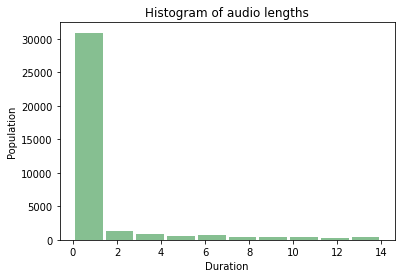
\includegraphics[width=0.9\textwidth]{./images/poly/duration.png}	
	\caption{Decision trees assembly only confusion matrix}
	\label{fig:poly_duration}
\end{figure}

\subsection{Feature Extraction}
\label{subsec:poly_feature}

\subsection{Model formulation}
\label{subsec:poly_model}



%----------------------------------------------------------------------------------------
%	SECTION 4
%----------------------------------------------------------------------------------------

\section{Experimental Results}
\label{sec:results}

\subsection{Monophonic results}
\label{subsec:mono_results}

\subsection{Polyphonic results}
\label{subsec:poly_results}

%----------------------------------------------------------------------------------------
%	SECTION 5
%----------------------------------------------------------------------------------------

\section{How to train NN on AMD GPU}
\label{sec:AMD}

%----------------------------------------------------------------------------------------
%	SECTION 6
%----------------------------------------------------------------------------------------

\section{Conclusions}
\label{sec:end}


%----------------------------------------------------------------------------------------
%	BIBLIOGRAPHY
%----------------------------------------------------------------------------------------

%\bibliographystyle{abbrv}
\bibliographystyle{unsrt}

\bibliography{bibliography}

%\nocite{*} % in case no ciattion was done or not all references has been cited 

%----------------------------------------------------------------------------------------


\end{document}